\section{Resultados y análisis}

\subsection*{Universidad de Moscow}

\subsubsection*{Recorrido en el Planisferio}

A continuación se puede ver de forma bastante clara como el paquete tuvo que pasar por estados unidos para luego ir a Europa Occidental hasta llegar finalmente a Rusia.

\begin{figure}[H]
  \centering
  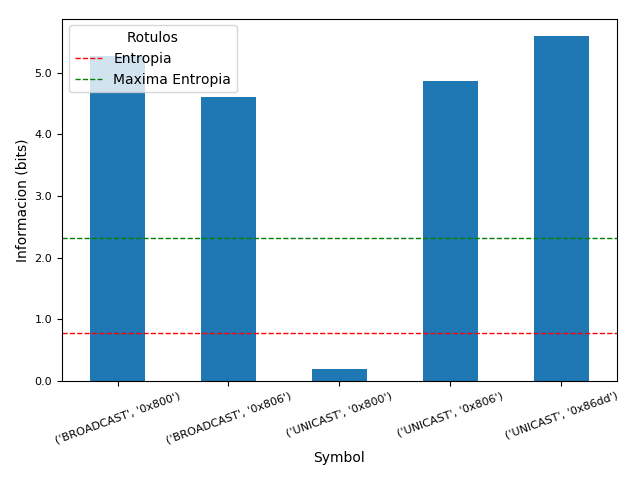
\includegraphics[width=8.5cm]{figs/information_hogar_ethernet_S1_output.png}
  \caption{\normalfont Recorrido realizado por los paquetes durante la ejecución de traceroute al intentar alcanzar el sitio www.msu.com}
\end{figure}

\subsubsection*{RTT entre saltos}

A continuación intentamos ver los timepos entre saltos. Para esto calculamos la media de cada de los RTTs obtenidos de cada TTL para reducir a solo un valor las mediciones obtenidas por cada TTL. 

Seguido de esto realizamos dos experimentos. Primero simplemente restamos los RTTs medios entre si como se puede ver en el primer gráfico, luego llevamos el experimento un paso mas allá normalizando con z-score los RTTs para eliminar cualquier tipo de deformación en las dimensiones del gráfico.

\begin{figure}[H]
  \centering
  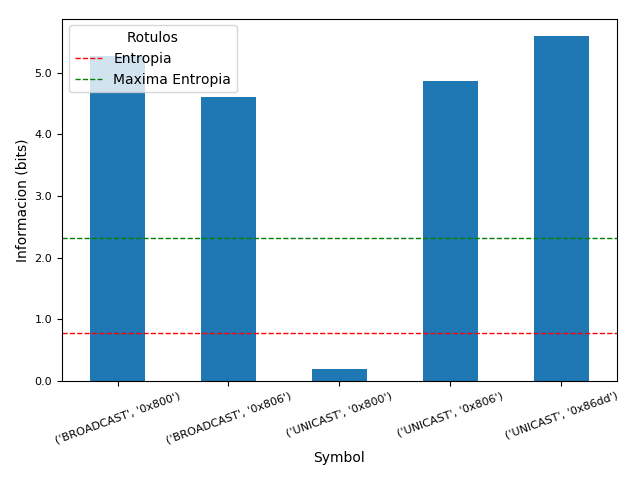
\includegraphics[width=8.5cm]{figs/information_hogar_ethernet_S1_output.png}
  \caption{\normalfont RTT entre saltos calculado a partir de restar los valores promediados a cada salto para el sitio www.msu.com}
\end{figure}

\begin{figure}[H]
  \centering
  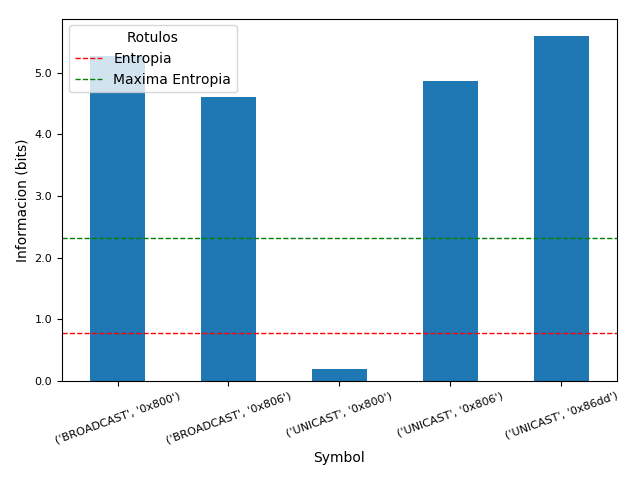
\includegraphics[width=8.5cm]{figs/information_hogar_ethernet_S1_output.png}
  \caption{\normalfont RTT entre saltos para el sitio www.msu.com calculado a partir de restar los valores promediados a cada salto y normalizarlos con z-score}
\end{figure}

Como se puede observar ... COMPLETAR.